\section{Methodology}
\label{sec:methodology}

We started from a lexical baseline based on Apache Lucene BM25 and progressively moved to a multi-stage neural pipeline.
Early experiments focused on analyzer choices, stopword lists, and BM25 variants; these runs were useful to establish a stable
baseline, but they also showed that lexical overlap alone is insufficient for this task.
\newline
We adopted a four-stage pipeline (Figure~\ref{fig:pipeline}) for our information retrieval system, consisting of:
\begin{itemize}
    \item \textbf{Query Translation}: queries in French or German are first translated into English.
    \item \textbf{Query expansion}: we expanded the English query with additional context to bridge the gap between informal and domain specific language.
    \item \textbf{Retrieval}: we retrieved relevant documents from the corpus using the expanded query.
    \item \textbf{Reranking}: we reranked the retrieved documents based on their relevance to the original query.
\end{itemize}
For each of these stages, we experimented with different models, chosing the ones that performed better in relation to the others.

In the following sections all the four stages are precisely explained.

\begin{figure}
    \centering
    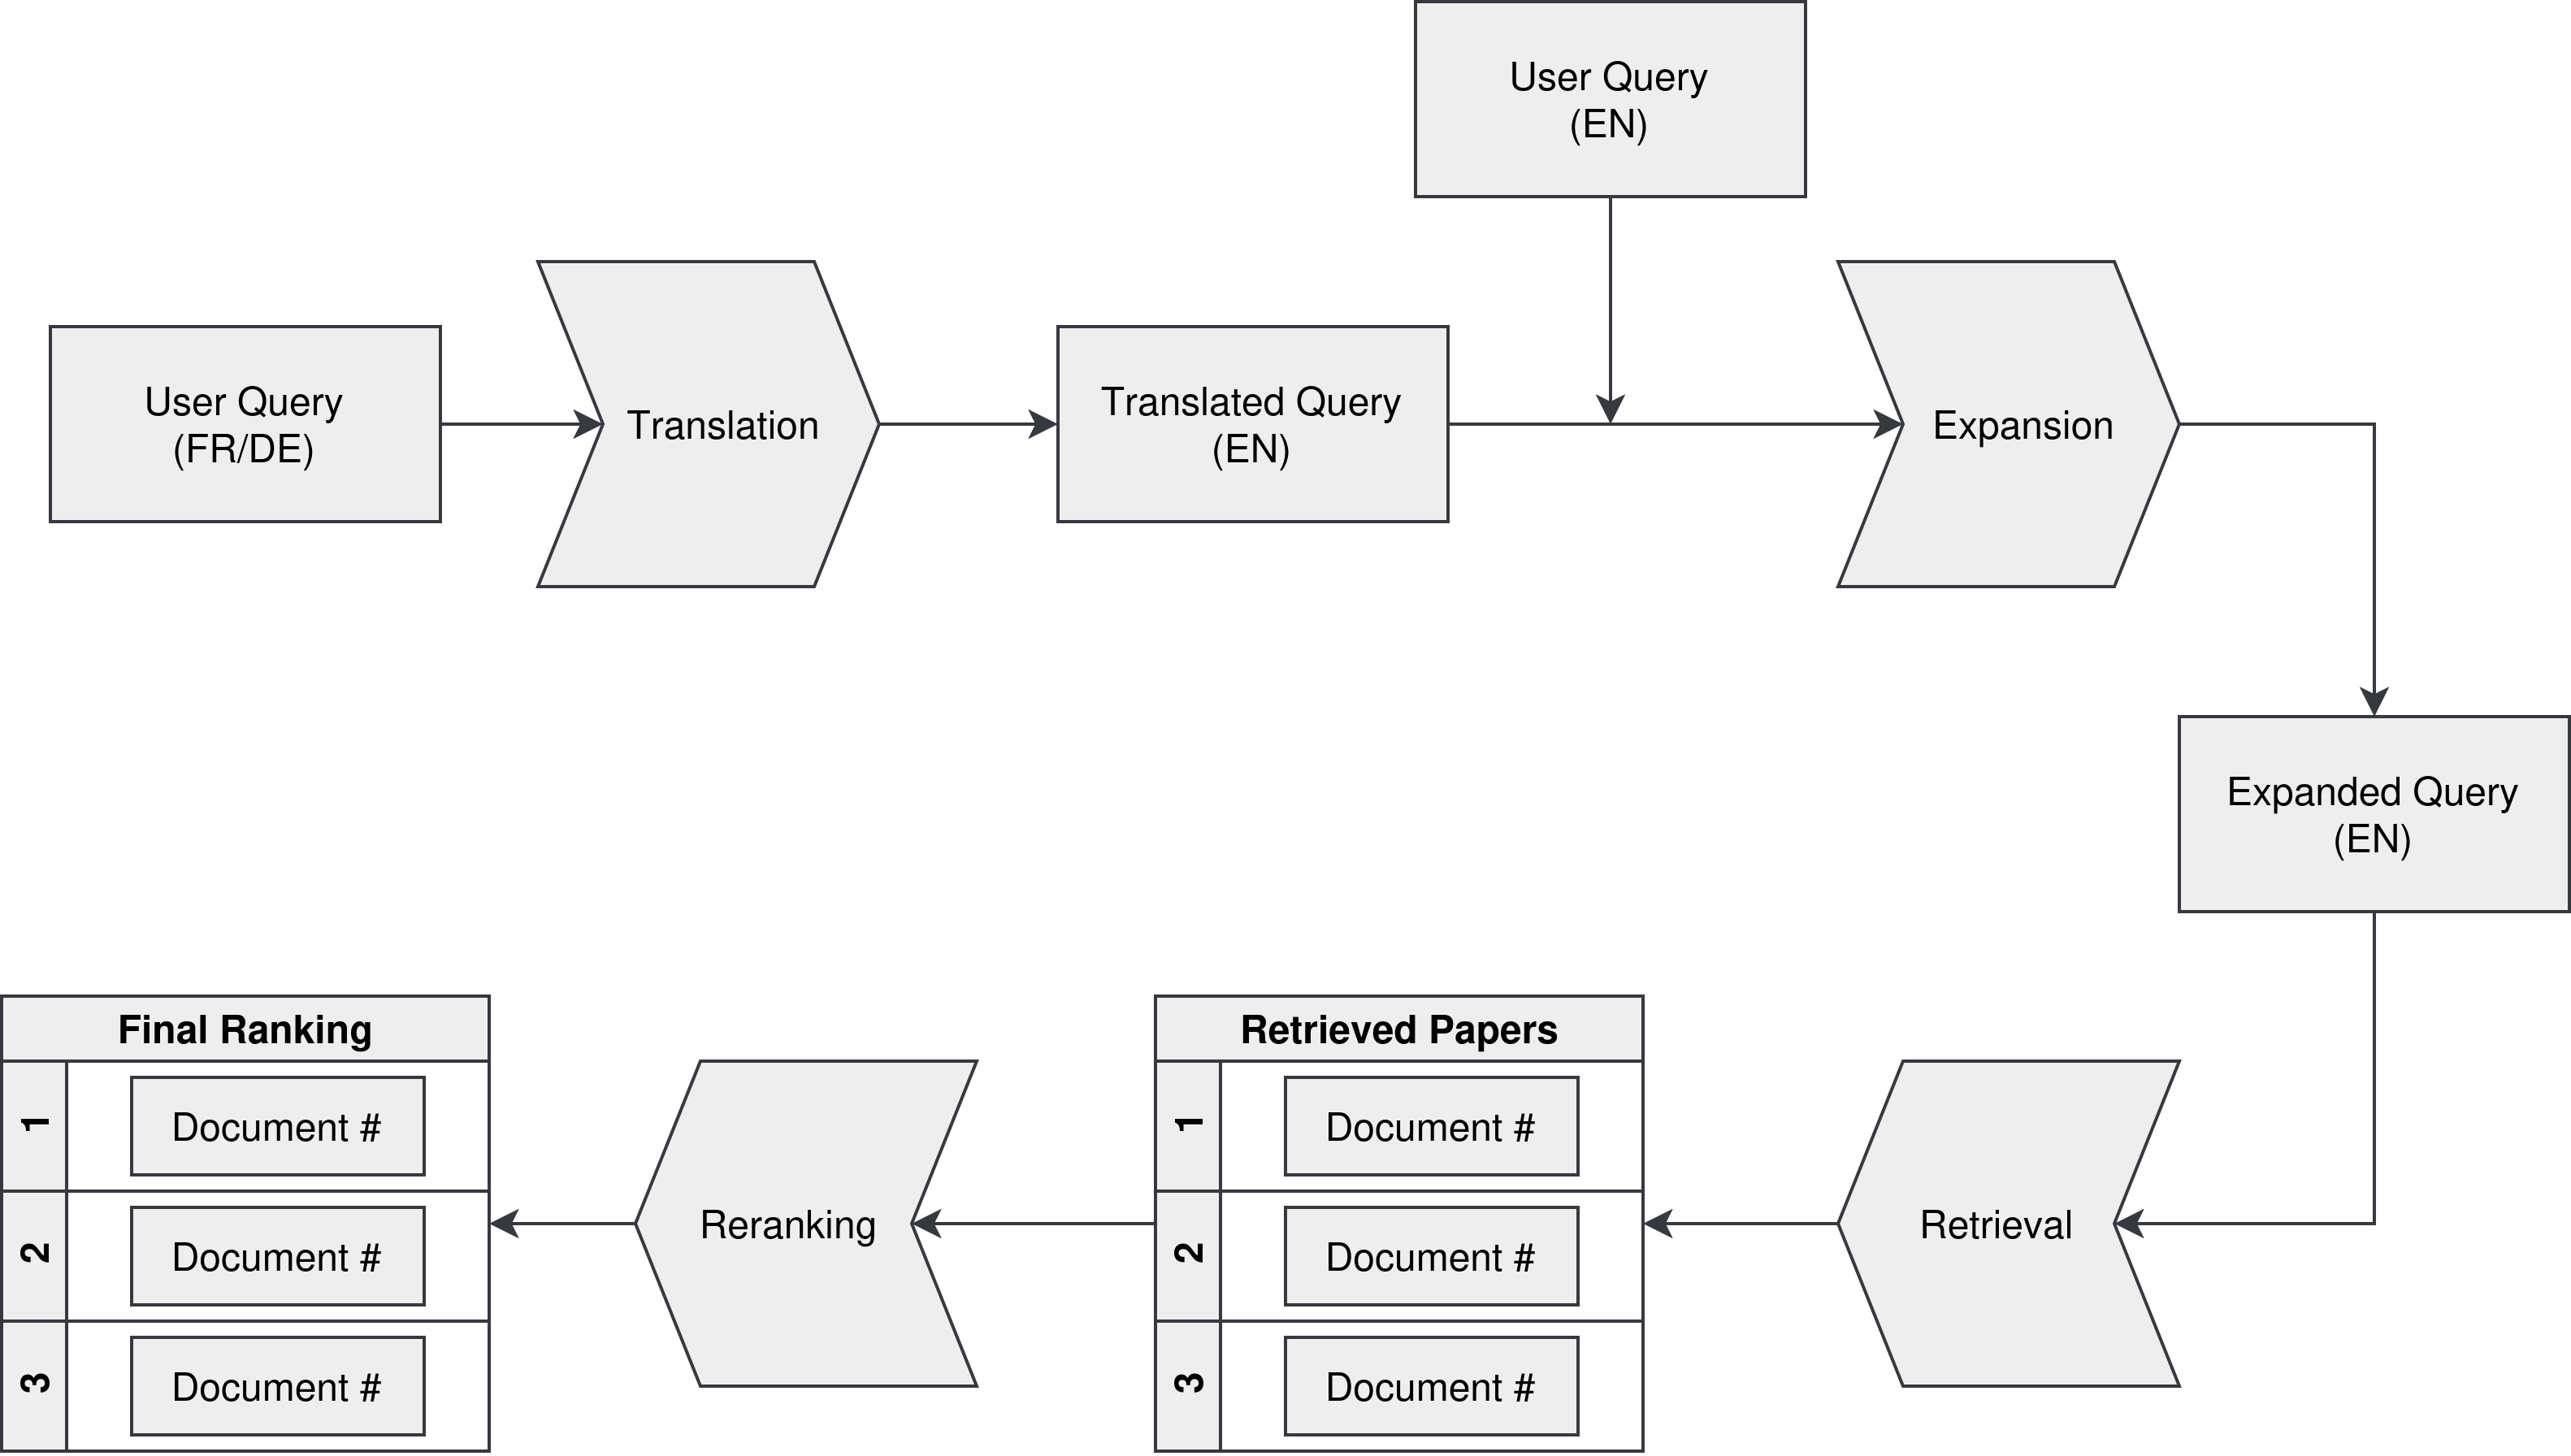
\includegraphics[width=0.8\linewidth]{figure/pipe.png}
    \caption{Four-stage pipeline for information retrieval.}
    \label{fig:pipeline}
\end{figure}

\subsection{Query translation} \label{sub:querytransl}
In the preliminary stage of out pipeline non-English queries (French and German) are translated into English. This is done query by query using the model \texttt{utter-project/EuroLLM-9B-Instruct-2512} with the following prompt:
\begin{promptbox}
\small
\ttfamily
\begin{flushleft}
\textit{system:} You are a professional translator.\\
Translate the user's text to English.\\
Output ONLY the English translation.\\
Do not include the original text, explanations, labels, or any other content.\\[0.8em]

\textit{user:} Translate this \{\textbf{French/German}\} text to English.\\
Output only the English translation, nothing else.\\[0.8em]

\{\textbf{Query original text}\}
\end{flushleft}
\end{promptbox}

The resulting English queries are then fed into the following step of our pipeline. 

\subsection{Query Expansion} \label{sub:queryexp}
Following the translation phase, the English queries undergo a semantic and lexical expansion process. This stage is designed to bridge the vocabulary gap between the user's informal query and the formal academic language present in the scientific document corpus. Unlike previous iterations that relied on generative LLM re-phrasings, the current architecture utilizes a hybrid expansion strategy, combining deep semantic retrieval with linguistic analysis. The expansion process follows three main technical steps:
\begin{itemize}
    \item \textbf{Keyword Extraction}: We use the \texttt{spaCy} library (\texttt{en\_core\_web\_sm}) to perform Part-of-Speech (POS) tagging on the translated query. We specifically extract nouns (\texttt{NOUN}) and proper nouns (\texttt{PROPN}), which represent the core technical entities of the claim.
    \item \textbf{Semantic Neighbor Retrieval}: The query is embedded using the \texttt{BAAI/bge-large-en-v1.5} model. We retrieve the top-5 most similar documents from the corpus to act as a source of domain-specific terminology. To ensure high-quality embeddings, we apply the BGE-specific instruction prefix: \textit{"Represent this sentence for searching relevant passages:"}.
    \item \textbf{Term Frequency Selection}: Candidate expansion terms are extracted from the retrieved neighbors and weighted based on their frequency and the original semantic similarity score.
\end{itemize}

The final expanded query is constructed by concatenating the original translated text, the extracted POS keywords, and the top-15 most relevant expansion terms. This creates a high-density representation that maximizes the probability of overlap during the hybrid retrieval stage, ensuring that both specific technical nomenclature and broader semantic contexts are represented. The resulting JSON object preserves the original query metadata while adding an \texttt{expanded} field for the downstream retrieval framework.


% After the translation (if needed), the queries undergo expansion: given the original query, we generate extra terms and tokens related to it.
% This serves two purposes: to increase the number of available tokens for a match, and to bridge the gap between the original
% informal query and the formal academic language used in the document corpus.\newline

Before confirming this as query expansion strategy, we have also tried to use two LLM models, \texttt{meta-llama/Llama-3.2-1B} and \texttt{openai/gpt-oss-20b} with the following prompt:
\begin{promptbox}
\small
\ttfamily
\begin{flushleft}
\textit{system:} ``Reasoning: \{reasoning\_effort\}''\\
You are a strict JSON-only retrieval query expansion generator.\\
Return the final answer only as valid JSON.\\[0.8em]

\textit{user:} You generate retrieval-specific query expansions.\\[0.5em]

Return only one valid JSON object with exactly these string fields:\\
\{\\
\hspace*{1em}``keywords'': ``\ldots'',\\
\hspace*{1em}``sparse'': ``\ldots'',\\
\hspace*{1em}``embedding'': ``\ldots'',\\
\hspace*{1em}``colbert'': ``\ldots'',\\
\hspace*{1em}``expanded'': ``\ldots''\\
\}\\[0.8em]

Rules:\\
-- Do not include markdown, code fences, emoji, commentary, arrays, or nested objects.\\
-- All five values must be strings.\\
-- Do not hallucinate facts.\\
-- Do not translate unless translation is already present in the query.\\
-- Preserve original-language terms.\\
-- \texttt{keywords}: compact important terms only; entities, nouns, technical terms, names, locations, dates, identifiers, acronyms, modifiers; no sentence.\\
-- \texttt{sparse}: lexical BM25/SPLADE-style expansion; exact-match terms, synonyms, acronyms, aliases, spelling and morphology variants; phrase fragments separated by spaces or semicolons; no long prose.\\
-- \texttt{embedding}: concise HyDE/query2doc-style natural-language semantic pseudo-document; include intent, context, and likely relevant-document framing.\\
-- \texttt{colbert}: concise late-interaction expansion; preserve important tokens and entities; add focused context and aliases; avoid synonym spam.\\
-- \texttt{expanded}: readable general-purpose merged expansion string combining the useful hints from the other fields.
\end{flushleft}
\end{promptbox}
This approach, which used a different expansion for each retrieval representation, did not improve performance. We therefore retained the simpler and more effective configuration based on a single expanded query. Section~\ref{sub:retrieval} describes in more detail how these expansion strategies were evaluated during retrieval.  
%Originally, we experimented with PRF-style expansion using semantic retrieval with \texttt{BAAI/bge-large-en-v1.5}.
% We then explored different methods for expansion,
% including Pseudo-Relevance Feedback (PRF) and similarity with static word embeddings using Word2Vec,
% testing these on both the original and the preliminary expanded queries.\newline

% In the final architecture, we used a multilingual LLM-based expansion script (\texttt{query\_expansion\_multilingual.py},
% default model \texttt{meta-llama/Llama-3.2-1B}) to generate multiple retrieval-oriented views of each query.
% The model is prompted to produce distinct representations,
% tailored to our multi-stage retrieval needs:
% \begin{itemize}
%     \item \textit{sparse}: A list of domain-specific keywords and technical synonyms (e.g., scientific nomenclature)
%     designed to maximize lexical overlap and mitigate the vocabulary mismatch in BM25-based retrieval.
%     \item \textit{dense}: A semantically enriched re-phrasing of the claim that provides a broader context, allowing the
%     bi-encoder in the next step of the architecture to produce more robust embeddings in the high-dimensional vector space.
%     \item \textit{ColBERT}: A structured, formal version of the claim (e.g., ``Serum levels and ICU admission'') that provides coherent
%     token sequences for fine-grained late-interaction scoring.
% \end{itemize}

% This multi-view expansion ensures that the downstream hybrid retriever can leverage both high-precision lexical matches
% and broad semantic overlaps. By generating these representations simultaneously within a single inference step of
% the same LLM,
% we maintain a coherent relationship between the different query ``views'', effectively providing a unified but multi-faceted
% context for the retrieval pipeline.\newline

% The resulting expanded queries are then fed into the multi-stage retrieval framework described next.

\subsection{Retrieval} \label{sub:retrieval}
The retrieval stage is designed as a high-recall candidate-generation step between query expansion and neural reranking. Its objective is not to make the final relevance decision, but to ensure that the true source paper is included in a sufficiently large candidate set for the subsequent, more computationally expensive cross-encoder stage. For this reason, after experimenting with a Lucene BM25 baseline, BGE-M3 using dense vectors only, and other bi-encoder models, the final pipeline adopts \textbf{BAAI/bge-m3} in a hybrid retrieval setting.

This choice reflects the nature of the task. Social media claims often contain informal paraphrases, hashtags, named entities, numerical values, and fragments of scientific terminology. Therefore, relying exclusively on exact lexical overlap or exclusively on dense semantic similarity may discard useful evidence. Hybrid retrieval is better suited to this setting because it combines complementary retrieval signals and can offer higher accuracy and stronger generalization capabilities~\cite{bge-m3}.

The retriever searches the fixed paper collection provided by the task organizers. Each paper is represented at document level by concatenating its title and abstract, and the retrieved unit is always the paper \texttt{pubkey}. We did not split papers into smaller chunks because the task requires identifying the source publication rather than retrieving a specific evidence passage. Using one representation per paper also avoids an additional chunk-to-document aggregation step. Although the collection includes metadata such as venue and authors, this hybrid retrieval stage uses only titles and abstracts, since these are the fields consistently encoded for all documents.

All input queries are converted into plain English, either because they are originally written in English or because they are translated before retrieval, see Section~\ref{sub:querytransl}. They are then expanded using the procedure described in Sections~\ref{sub:queryexp}.

We chose \textbf{BAAI/bge-m3} because it is well suited to this retrieval setting. The model can produce dense vectors, sparse lexical weights, and ColBERT-style multi-vector representations from the same encoder. This allows the retriever to combine broad semantic matching, exact term evidence, and fine-grained token-level matching without switching between unrelated encoders.

Candidate selection is performed in two steps. First, all documents are encoded as dense BGE-M3 vectors and searched with an inner-product FAISS index~\cite{faiss_documentation}. This dense stage acts as an efficient broad filter over the whole collection. The default setting retrieves a large candidate pool of \texttt{candidate\_multiplier} $\times$ \texttt{top\_k}, with \texttt{candidate\_multiplier = 3} and \texttt{top\_k = 2000}, before the final truncation. This deliberately large candidate set favours recall, which is more important than precision at this stage.

Second, the dense candidates are rescored using the sparse and ColBERT-style representations. The sparse component rewards important overlapping terms, while the ColBERT-style component captures local token correspondences that may be lost when each document is represented by a single dense vector~\cite{KhattabZaharia2020}.

The final configuration was selected through a series of development runs. We first tuned the lexical baseline by varying the Lucene analyzer, stop-word lists, stemming strategy, and BM25 searcher variants. These experiments improved the classical baseline, but also highlighted its limitations for this task: even with query expansion and reranking, BM25-based candidate generation remained more dependent on surface-level lexical overlap than desired.

We then evaluated dense retrieval with several bi-encoder models. Among these, \textbf{BAAI/bge-m3} achieved the strongest performance and improved the semantic coverage of the candidate set, particularly for paraphrased and multilingual claims. We also tested BGE-M3 in a hybrid retrieval setting, using a setup that differed slightly from the final configuration. In those experiments, sparse, dense, and ColBERT-style retrieval were performed using dedicated query expansions tailored to each retrieval mode. More specifically, each query was represented through three complementary views: an embedding view for semantic matching, a sparse view for lexical and term-based evidence, and a ColBERT view for fine-grained token-level interaction.

However, the best results in our analysis were obtained with a simpler configuration in which BGE-M3 hybrid retrieval used the same expanded query, described in the previous section, for all three retrieval modes. We then tested several weighting configurations. Among them, the run labelled \texttt{bge\_m3\_hybrid\_513} was retained because it provided the strongest recall-oriented trade-off among the retrievers evaluated without reranking. This configuration used weights of $0.5$, $0.15$, and $0.35$ for dense, sparse, and ColBERT scoring, respectively, with a multiplier of $3$ and a maximum hybrid input length of $384$.

A closely related configuration with a larger ColBERT weight achieved a nearly identical MRR@5, but a lower Recall@100. We therefore preferred the configuration that better matched the role of retrieval as a candidate generator. This choice was further confirmed by downstream experiments: reranking candidates from \texttt{bge\_m3\_hybrid\_513} consistently outperformed the corresponding BM25-based reranked runs. In addition, increasing the reranked candidate depth from a few hundred documents to between $1000$ and $2500$ documents improved the final recall available to the reranker.

We also experimented with a learned fusion strategy for the hybrid signals. In particular, the experimental setup included a LightGBM LambdaMART option that builds features from the dense, sparse, and ColBERT scores, together with normalized score variants and dense-rank features, and then learns how to combine them. However, the retained retrieval configuration uses simpler linear fusion, which is easier to reproduce and aligns well with the recall-oriented role of this stage.

The final hybrid retrieval score is therefore computed as:
\[
s(q, d) =
0.5\,s_{\text{dense}}(q, d)
+ 0.15\,s_{\text{sparse}}(q, d)
+ 0.35\,s_{\text{colbert}}(q, d).
\]

The largest weight is assigned to the dense score because it provides the main semantic signal. The sparse and ColBERT components add complementary lexical and fine-grained matching evidence. Candidates are sorted by this score in descending order and truncated to the final \texttt{top\_k}. The retrieval output is a JSON mapping from each query ID to an ordered list of paper \texttt{pubkeys}. Scores are not exported, because the next stage treats retrieval as a candidate generator and recomputes relevance using a cross-encoder over the returned document identifiers.


\subsection{Reranking} \label{sub:reranking}

The reranking stage receives the candidate list produced by the hybrid retriever and reorders it with cross-encoders.
Its goal is to improve early precision (especially MRR@5) while preserving as much recall as possible from the first stage.

Our strongest single-stage reranker is \texttt{nvidia/llama-nemotron-rerank-1b-v2}. For each query--document pair,
we build an input sequence with the template \texttt{question: \{q\}} followed by \texttt{passage: \{p\}} and compute a scalar relevance
score with a sequence-classification head. Documents are then sorted by this score.
In practice, reranking deeper candidate pools (e.g., 500--1000 documents) gave better final results than shallow pools,
confirming the importance of high recall before neural ranking.

We also evaluated alternative rerankers, including Qwen3 and GTE-ModernBERT variants, and tested cascaded reranking.
In the best cascaded configuration, Nemotron is used as the first reranking pass and a second reranker
(\texttt{BAAI/bge-reranker-v2-m3} or a fine-tuned \texttt{ModernBERT-large}) refines the top portion of the list.
This two-step reranking improves top-rank ordering over single-stage reranking.

\subsection{Evaluation}

We evaluate systems on the CheckThat! Task 1 query sets by matching retrieved \texttt{pubkey}s against the gold \texttt{pubkey}
for each query. The official optimization target is MRR@5, which we use as the primary score during model and parameter
selection. In parallel, we track Recall@100 to monitor candidate-generation quality and to verify that reranking gains do not
come from overly aggressive filtering.

For internal analysis, our evaluator also computes additional ranking metrics (e.g., Recall@1/5/10/100, Precision@1/5/10,
MAP, and nDCG@k). This broader view is useful to interpret trade-offs between recall-oriented retrieval settings and
precision-oriented reranking settings, while keeping MRR@5 as the main criterion for reporting and model selection.
